\chapter{CN-VIP}\label{chap:cn-vip}

\margintoc{}

I already mentioned some of the typing rules related to memory actions and
pointer operations in \nameref{sec:kernel-mem-action-ops}, but I can now
recapitulate them with more detail, drawing special attention to parts about
liveness and bounds checks I skimmed past before. For convenience, I have
reproduced \cref{fig:typing-mem-action} in \cref{fig:cnvip-mem-action}.

\section{Memory actions}

\begin{figure*}[tp]
    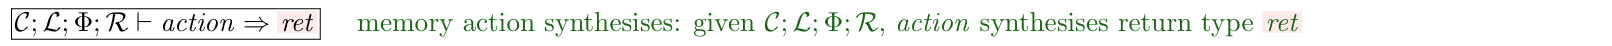
\includegraphics{figures/kernel-mem-action-typing-1}
    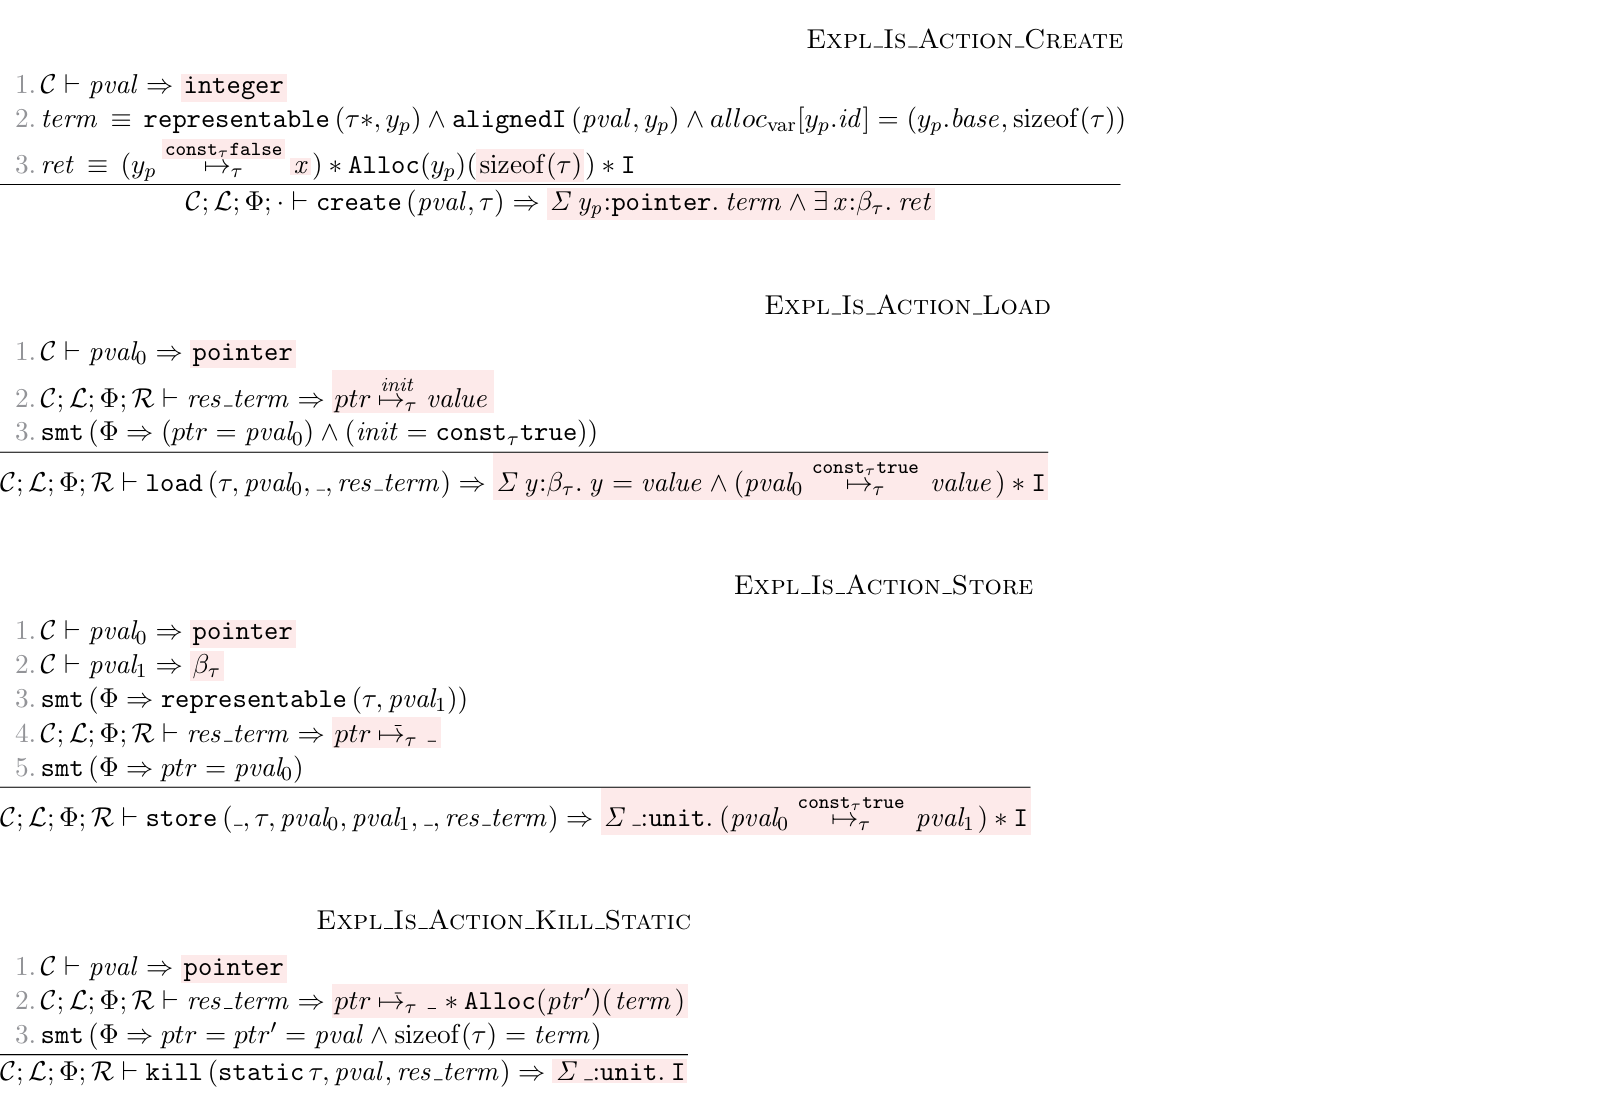
\includegraphics{figures/kernel-mem-action-typing-2}
    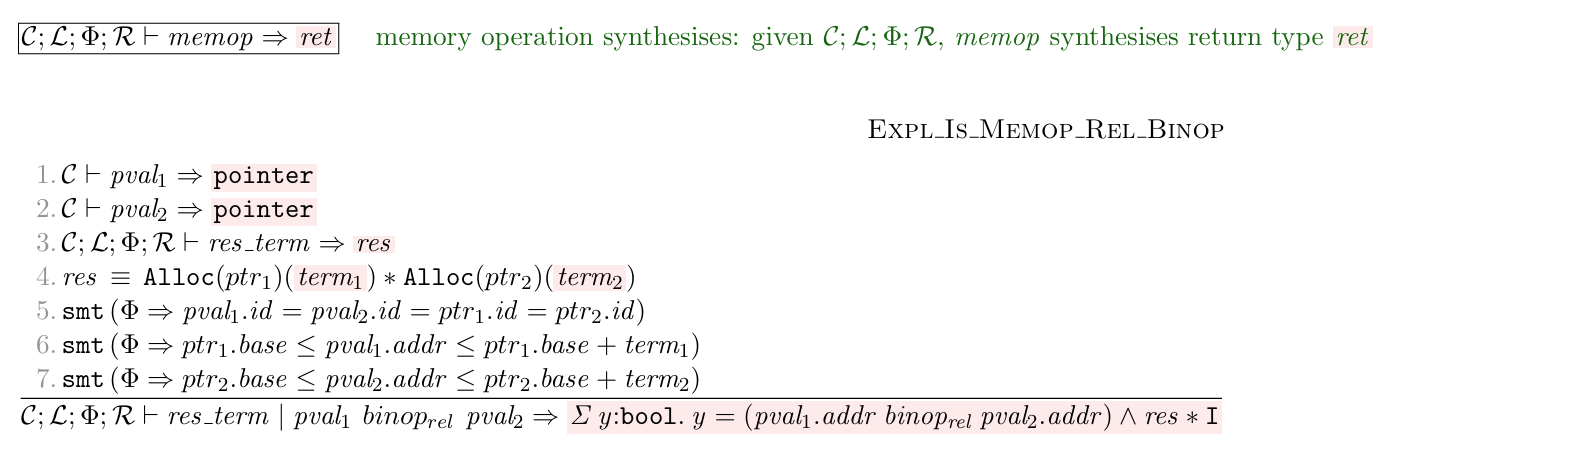
\includegraphics{figures/kernel-memop-typing}
    \caption{\kl{Kernel CN} typing rules for memory actions, and a select rule
        for typing a memory operation.}\label{fig:cnvip-mem-action}
\end{figure*}

In \textsc{Expl\_Is\_Action\_Create}, creating an allocation produces new
constraints on its base address and size. These are tracked via constraints on a
logical variable $\mathit{alloc}_\mathrm{var}$, a map from \kl{allocation ID}s to
pairs of a base address and size. This can simply be interpreted as an implicit
logical argument and return value for each function call.\sidenote{Need to
check the typing rules to ensure enforce this idea consistently.} Creating an
allocation also produces an \cninline{Alloc} token, to track the fact the
allocation is live, as well as the usual ownership/points-to resource.

TODO\@. Having a memory model also allows me to introduce support for dynamic
memory management. Whereas the above rule is only defined for typed objects
such as locals or globals, a region is essentially just an array of memory
bytes. For simplicity, I model every allocation as succeeding, so that the
pointer returned is never \cinline{NULL}. Hence the typing rule is similar,
but instead of ownership of a single object at a given C type, the ownership
is an iterated one over an array of memory bytes.

Conversely, in \textsc{Exp\_Is\_Action\_Kill}, destroying an allocations
requires both ownership of it (remember ownership represent read/write
permissions, but not allocation and freeing permissions), and the
\cninline{Alloc} token, plus proof that the given pointer is the same as the
owned pointer, and has the same base address as indicated by the allocation
token. For static kills (a block variable going out of scope), the rule also
checks that the size of the C type is also the size of the allocation.
TODO\@. Destroying a region is similar, except with an iterated ownership
of memory bytes.

Fortunately, the rules for loads and stores do not change at all. Ownership of
a location is enough to deduce that the allocation is live, and I assume
ownership is guaranteed to be in bounds for any allocation.\sidenote{Ownership
of out-of-bounds resources is equivalent to $\mathsf{false}$.}

\section{Pointer operations}

There are large discrepancies between the rules for pointer offsets presented
in \sidetextcite{lepigre2022vip} and \sidetextcite{memarian2022cerberus}, and
the \kl{Cerberus source code}, which I have detailed in a table in
\cref{fig:offset-confusion}. I am awaiting clarification on the correct way to
proceed.

\begin{figure*}[tpb]
  \begin{tabular}{ccccc}
  \toprule
   & \citeauthor{lepigre2022vip} incl.\ appendix & \citeauthor{memarian2022cerberus} & Cerberus code \\
  \midrule
  Member (P)
    & {\checksymbol✗}
    & case \cinline{NULL}
    & case \cinline{NULL}, 0-offset
  \\
  Member (ISO)
    & bounds, case 0-offset
    & bounds, liveness
    & case \cinline{NULL}, 0-offset
  \\
  Array (P)
    & {\checksymbol✗}
    & \textendash{}
    & \textendash{}
  \\
  Array (ISO)
    & bounds
    & bounds, liveness
    & bounds, liveness
  \\
  \bottomrule
  \end{tabular}
  \caption{Rules for computing pointer offsets (member and array, with
      pure/permissive (P) and ISO variants) in PNVI-ae-udi, across three
      different sources. `{\checksymbol✗}' means the rule is omitted. `case'
      means the rule special cases on that value. `\textendash{}' means
      there are no checks. `bounds' means a bounds check on the resulting
      pointer. `liveness' means a liveness check on the allocation.}\label{fig:offset-confusion}
\end{figure*}

Pointer operations such as taking the difference between two pointers or
relational comparison between two pointers, require both pointers to be in
bounds of the same live allocation. Hence the rule in\sidenote{TODO fix the
rule, which is very wrong in many ways} \cref{fig:cnvip-mem-action} ask
asks the solver to prove (a) the \kl{allocation ID}s are equal (b) that the
pointer are within bounds of the allocation (c) to check there exists a
live allocation with that ID\@. The evidence of a live allocation can be
either ownership with the same \kl{allocation ID}, or an \cninline{Alloc} token,
and the rule is agnostic as to which, just that this evidence is returned
in the type so as to not consume/destroy it.

A rule that is present in the code, but missing in other formats for
\kl{PNVI-ae-udi} is that for casting pointers to dead allocations to integers,
which is permitted so long as the address can fit within the target integer
type. Since \kl{VIP} does not track exposure, the live and the dead
pointer cases collapse into the same case. On top of this, as I mentioned in
\cref{subsec:prov-int-bytes}, I chose to support the limited provenance in
integers required via a new C type, to make the any additional complexity and
performance cost as opt-in, and to avoid changing all the base types for
integers of various sizes (bit vectors) to a datatype with two constructors.
Because of these two simplifications, the cast is therefore just an identity,
on the SMT term and its base type.\sidenote{TODO add this rule} The rules for
casting an integer to a pointer is \kl{UB} if it is not in the \cinline{NULL}
or round-trip case, and is an identity in the latter.\sidenote{TODO add
this rule} And the rule for \cinline{copy_alloc_id} performs a bounds check on
the integer using the \kl{allocation ID} supplied by the pointer, and combines the
two into a new pointer.\cinline{TODO add this rule too}

The new C types need to be handled with care to implement the subtyping
required for a smoother experience.\sidenote{TODO figure out the subtyping
for base types and resources\ldots}

\section{\cinline{memcpy} and \cinline{memcmp}}

The typing rules for \cinline{memcpy} require iterated ownership of two
contiguous arrays of \kl{memory bytes} of length $n$; it returns ownership of
both, with the constraint that the value of the destination (first) is equal to
that of the source (second). The iterations must be contiguous and of the same
length to express the equality constraint on the values correctly.

The typing rules for \cinline{memcmp} require iterated ownership of two
contiguous arrays of \kl{memory bytes} of length $n$; like \cinline{memcpy}, it
returns ownership of both, unlike \cinline{memcpy} its resulting value is not
straightforward to specify, because the concise or obvious specification would
use quantifiers. I refer to a recursively defined logical function which
constrains the result to be (a) unconstrained if it reads any
\coreinline{unspec} values (b) 0 if all bytes (excluding provenances) are equal
and (c) the difference between the first two unequal bytes otherwise. The presence
of \coreinline{unspec} values makes it difficult to give a simpler specification
to the result such as \cninline[breaklines]{src == dest && result == 0i3 || src
!= dest && result != 0i32}, because we want to do not wish to imply % chktex 26
\cninline{unspec == unspec}.\sidenote{The simpler specification could be
achieved with a notion of \emph{comparable bytes}, converting to which would
require ownership of only initialised and non-padding bytes.}

Both of these typing rules require a way to get ownership of memory bytes, for
which, \kl{CN-VIP} adds new annotations.\sidenote{TODO add these typing rules}
In the formal presentation, these are represented by operations on predicates
which consume ownership of an object, and produce ownership of memory bytes, or
vice versa.

\section{Soundness}\label{sec:cn-vip-soundness}

There are few steps involved to updating the formalisation to use a \kl{VIP}
based memory object model from its current concrete one.
\begin{enumerate}
    \item Extend the configuration of the dynamic semantics to be a step
        relation between abstract \emph{states} and expression, rather than
        just \emph{heaps} and expressions.
    \item Extend the heap typing rules to incorporate the newly added
        allocation history.
    \item Update the proof of soundness for resource term reduction and pattern
        matching, with the new rules.
    \item Define an interpretation of heaps in ResCore, to heaps in the CN-VIP
        memory model.
    \item Prove that the ResCore model of heaps is sound with respect to
        \kl{PNVI-ae-udi}, perhaps via an intermediate concrete memory model.
\end{enumerate}

\subsection{Extending the dynamic semantics}

In the typing rules, I modelled the allocation history as a single global
logical variable $\mathit{alloc}_\mathrm{var}$. This means that even morally
closed programs have that variable free in explicit logical and resource terms.
At the same time, because the allocation history is extended during the course
of evaluating a \kl{ResCore} program, it is not a term which can be substituted
once at the start of the program and close. Hence, the allocation history must
be threaded through to any part of dynamic semantics which relies on checking
constraints (in the empty context) using the SMT solver. At the point of
calling, the allocation history is substituted in, with the most up to date
information, to check the constraint as a closed term (\cref{fig:mem-model-dyn-smt}).

\begin{marginfigure}
    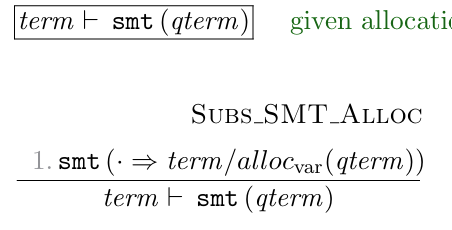
\includegraphics{figures/mem-model-dyn-smt}
    \caption{Calls to the SMT solver are now extended to thread through the
        changing allocation history.}\label{fig:mem-model-dyn-smt}
\end{marginfigure}

Only the \coreinline{create} memory action extends the allocation history, and
so it and every grammar node containing it also includes the allocation history
as part of its configuration, rather than threaded through the
side.\sidenote{TODO fix premise 7 of the create dynamic rules.} Note that
because I split the intuitionistic part of the allocation history from the
linear part, it does not get updated to record a dead allocation in the
rule for \coreinline{kill} (\cref{fig:mem-model-dyn-create-kill}).

\begin{figure*}
    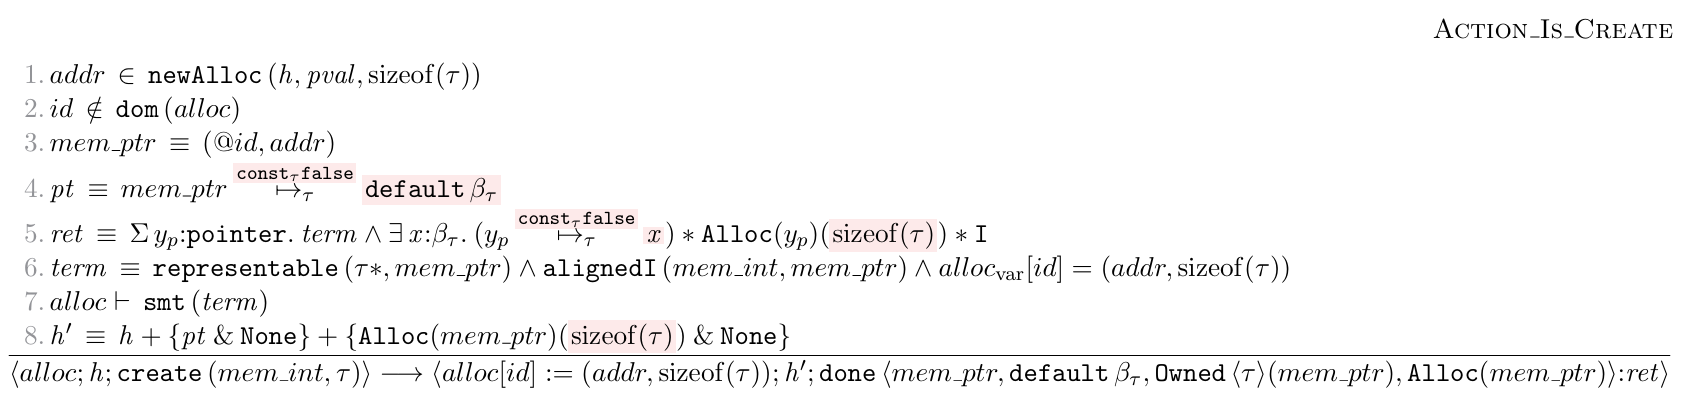
\includegraphics{figures/mem-model-dyn-create}
    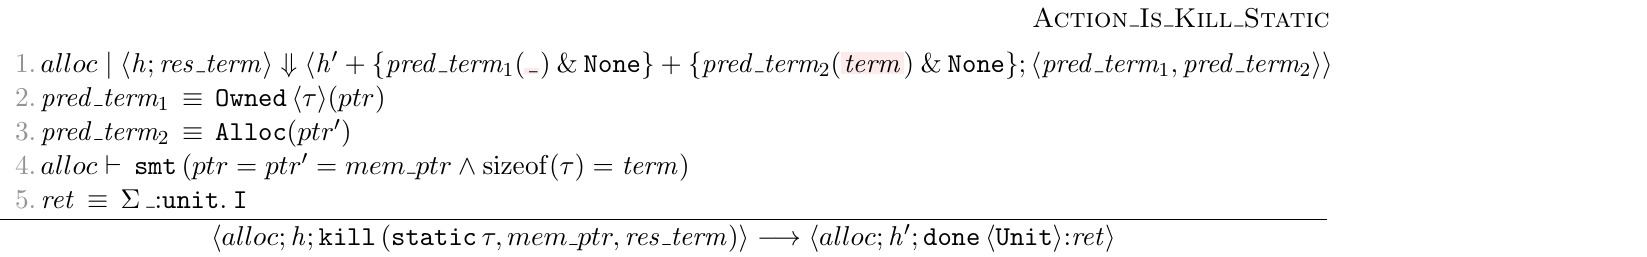
\includegraphics{figures/mem-model-dyn-kill}
    \caption{The allocation history only tracks a mapping from IDs to a pair of
        base address and size, so when an allocation is killed, existing entries
        are not mutated.}\label{fig:mem-model-dyn-create-kill}
\end{figure*}

With the exception of threading through the allocation history, the rules for
loads and stores are unchanged. The rules for converting ownership of objects
into iterated ownership of memory bytes and vice versa are predicate
operations, much like the ones for manipulating structs and fixed-length
arrays.\sidenote{TODO add them} The rules for \coreinline{memcpy} and
\coreinline{memcmp} are also as expected.\sidenote{TODO add them}

Pointer operations do not extend the allocation history, but do require the
heap to check whether the supplied pointers belong to live allocations. They
are agnostic of whether it is ownership or an \cninline{Alloc} token is
provided as evidence (\cref{fig:mem-model-dyn-ptr-relop}).\sidenote{TODO
add/fix this}

\begin{figure*}
    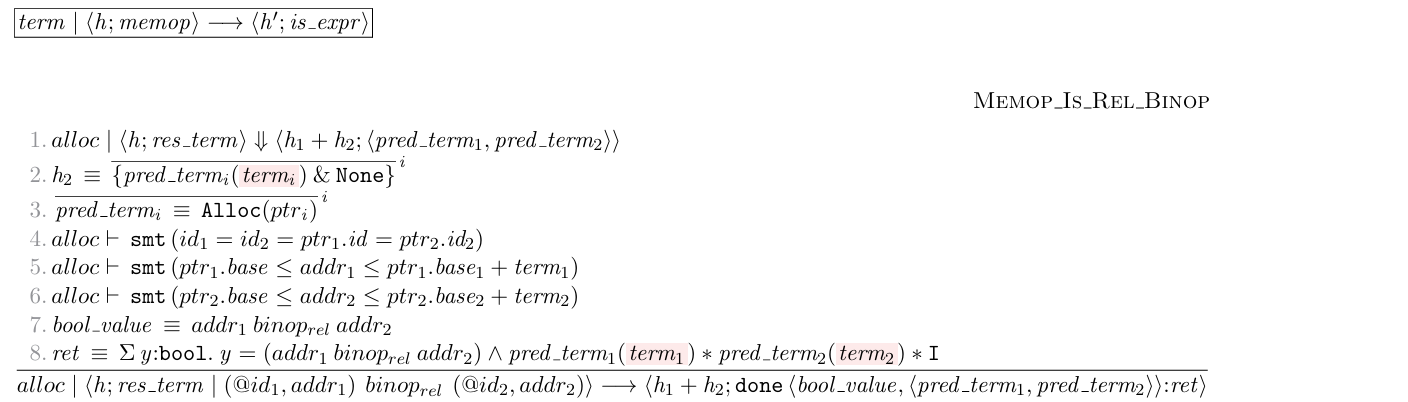
\includegraphics{figures/mem-model-dyn-ptr-relop}
    \caption{Memory operations involving pointers perform a bounds check using
        the SMT solver and supplied pointers, and a liveness check based on
        evidence from the supplied resource term and the heap.}\label{fig:mem-model-dyn-ptr-relop}
\end{figure*}

Lastly, there are the rules about pointer to integer casts, integer to pointer
casts and the \cinline{copy_alloc_id} primitive. The latter two check that that
resulting pointer is in the bounds of a live allocation; they are also agnostic
as to whether it is ownership or an \cninline{Alloc} token which is provided as
evidence.\sidenote{TODO this too\ldots}

\subsection{State typing}

Because the abstract state now includes an append-only allocation history, the
typing rules for heaps (\cref{sec:heap-types}) needs to be generalised to
include it. The main judgement involved in this is $\mathit{alloc} \Leftarrow
\Phi$, which says that the allocation history $\mathit{alloc}$ is consistent
with constraint context $\Phi$. \cref{fig:alloc-typing} shows that it does so
by checking if each constraint, with the allocation history substituted for the
$\mathit{alloc}_\mathrm{var}$, holds (under the empty context).

\begin{marginfigure}
    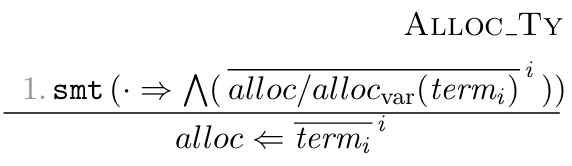
\includegraphics{figures/alloc-typing}
    \caption{Definition of a well-constrained allocation history \textemdash{}
        $\mathit{alloc}$ is consistent with each constraint in context
        $\Phi$.}\label{fig:alloc-typing}
\end{marginfigure}

The heap typing rule generalises similarly (\cref{fig:heap2-typing}). It
substitutes the allocation history for $\mathit{alloc}_\mathrm{var}$, and then
types the heap exactly as before.

\begin{marginfigure}
    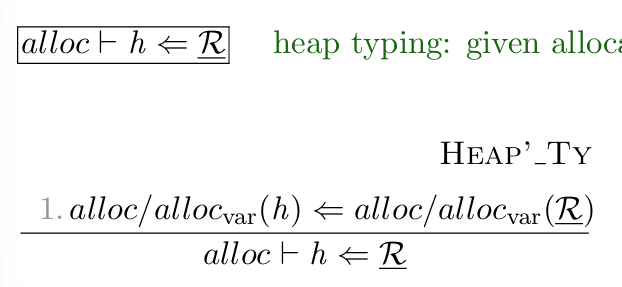
\includegraphics{figures/heap2-typing}
    \caption{Definition of heap typing in the presence of a allocation history:
        substitute the history into the heap and the type (\kl{normalised}
        resource context) and type as before.}\label{fig:heap2-typing}
\end{marginfigure}

\subsection{Updating the soundness proof}

Recall that I defined resource term reduction and pattern matching in the
dynamic semantics in a big-step style (\cref{sec:heap-types}). Whilst this
intertwines the proofs for progress and type preservation, its advantage of
modularity pays off now. The new constructs such as non-deterministic pointer
equality, \coreinline{allocate_region}, \coreinline{kill_dynamic},
\cinline{memcpy}, \cinline{memcmp}\cinline{copy_alloc_id}, and the conversions
to and from memory bytes, are just additional cases in the proof, the rest are
merely updates. The updates are small because the additional the additional
constraints on the allocation history are easy to link across the static and
dynamic semantics by the definition of allocation history typing. The bounds
and liveness checks are similarly easy to link across the static and dynamic
semantics by the definition of heap typing. The updated theorem statements are
as below: the main differences are the use of the updated abstract state typing
judgements, and the use of the $\mathcal{L}_0 = {\; \mathit{alloc}_\mathrm{var}
\;}$ environment, instead of the empty one, for logical variables. Updated
proofs are in the appendix.

\begin{theorem}[CN-VIP:\ progress and type preservation for resource terms]
For all resource terms ($[[ res\_term ]]$) closed which type check or synthesise
($[[ cdot ; L0 ; N ; nR |- res\_term <= res ]]$), and well-typed states
($[[ alloct ; h <= N ; nR ]]$), there exists a resource value ($[[ res\_val ]]$),
context ($[[ nR' ]]$) and heap ($[[ h' ]]$), such that: the value is well-typed
($[[ cdot ; L0 ; N ; nR' |- res\_val <= res ]]$); the heap is well-typed
($[[ alloct |- h' <= nR' ]]$), and for all frame-heaps ($[[ f ]]$), the resource term
reduces to the resource value without affecting the frame-heap
($[[ alloct | < h + f ; res\_term > ||v < h' + f ; res\_val > ]]$).
\end{theorem}

\begin{theorem}[Progress for the annotated and let-normalised Core]
If a top-level expression ($[[ texpr ]]$) is well-typed
($[[ cdot ; L0 ; N ; nR |- texpr <= ret ]]$) and all computational patterns
in it are exhaustive, then either it is a value ($[[ tval ]]$), or it is
unreachable, or for all well-typed states ($[[ s <= N ; nR ]]$)
then there exists another state ($[[ s' ]]$) and expression ($[[ texpr' ]]$)
which is stepped to ($[[ < s ; texpr > --> < s' ; texpr' > ]]$)
in the operational semantics.
\end{theorem}

\begin{theorem}[Type preservation for the annotated and let-normalised Core]
For all closed and well-typed top-level expressions
($[[ cdot ; L0 ; N ; nR |- texpr <= ret ]]$),
well typed states ($[[ alloct ; h <= N ; nR ]]$),
frame-heaps ($[[ f ]]$),
new states ($[[ alloct' ; h' ]]$),
and new top-level expressions ($[[ texpr' ]]$),
which are connected by a step in the operational semantics
($[[ < alloct ; h + f ; texpr > -->  < alloct' ; heap ; texpr' > ]]$),
if all top-level functions are annotated correctly,
there exists a constraint context ($[[ N' ]]$),
sub-heap ($[[ h' ]]$),
and resource context ($[[ nR' ]]$),
such that the constraint context is extended
($[[ cdot ; L0 ; N ; cdot \sqsubseteq cdot ; L0 ; N' ; cdot ]]$),
the frame is unaffected ($[[ heap ]] = [[ h' + f ]]$),
the sub-state is well-typed ($[[ alloct' ; h' <= N' ; nR' ]]$),
and the top-level expression too
($[[ cdot ; L0 ; N' ; nR' |- texpr' <= ret ]]$).
\end{theorem}

\chapter{Implementation of CN-VIP}

\margintoc{}

In addition to designing, formalising, and proving it sound, I also implemented
CN-VIP\@. This was a substantial project which I worked on for about seven
months, from August to October of 2023, and May, June, Septemeber and October
of 2024.\sidenote{See
    \href{https://github.com/search?q=repo\%3Arems-project\%2Fcerberus+author\%3Adc-mak\&type=commits\&s=committer-date\&o=asc}{my commits}
    to the \kl{Cerberus} repository. In the intervening months, I
    worked on a failed update to the buddy allocator of pKVM to work with
    bitvectors (\cref{chap:buddy}), engineering for accurate source location
    information (\cref{sec:error-msgs}), and MiniCN (\cref{chap:kernel-alternative}).}

What made it more challenging was that it had to be developed and integrated
piecemeal alongside other active \kl{CN} development.

The first step was adding in the various pieces of infrastructure in a non-functional way.
\begin{itemize}
    \item A logical variable for allocation history.
    \item A resource predicate for the \cninline{Alloc} token and using them in
        \coreinline{create} and in \coreinline{kill}.
    \item Additional constructs like \cinline{copy_alloc_id}.
    \item A datatype for the SMT representation of pointers, instead of integers.
    \item A flag to ensure changes to the pointer representation could be toggled on or off.
    \item Deprecating integer to pointer casts in the specification language.
    \item Adding array and member shifting operators.
\end{itemize}

Given all this, the next steps were about implementing support for bounds and
liveness checks, which was relatively straightforward.
\begin{itemize}
    \item Adapt and categorise the PNVI/VIP test suite to CN VIP\@.
    \item Support for non-deterministic pointer equality.
    \item Add a pointer liveness check.
    \item Add bounds checks, sometimes dependent on pointer liveness.
    \item Add basic support for \cinline{memcpy} (no provenance or
        \coreinline{unspec} values).
\end{itemize}

At this stage of development, I switched on CN-VIP by default, but retained the
ability to switch it off behind a flag. Fortunately, this happened just after
benchmarking on the CN tests was added, so we have a measurement of the impact
of the transition, shown in \cref{fig:vip-performance-hit}.

\begin{figure}[h]
    \centering
    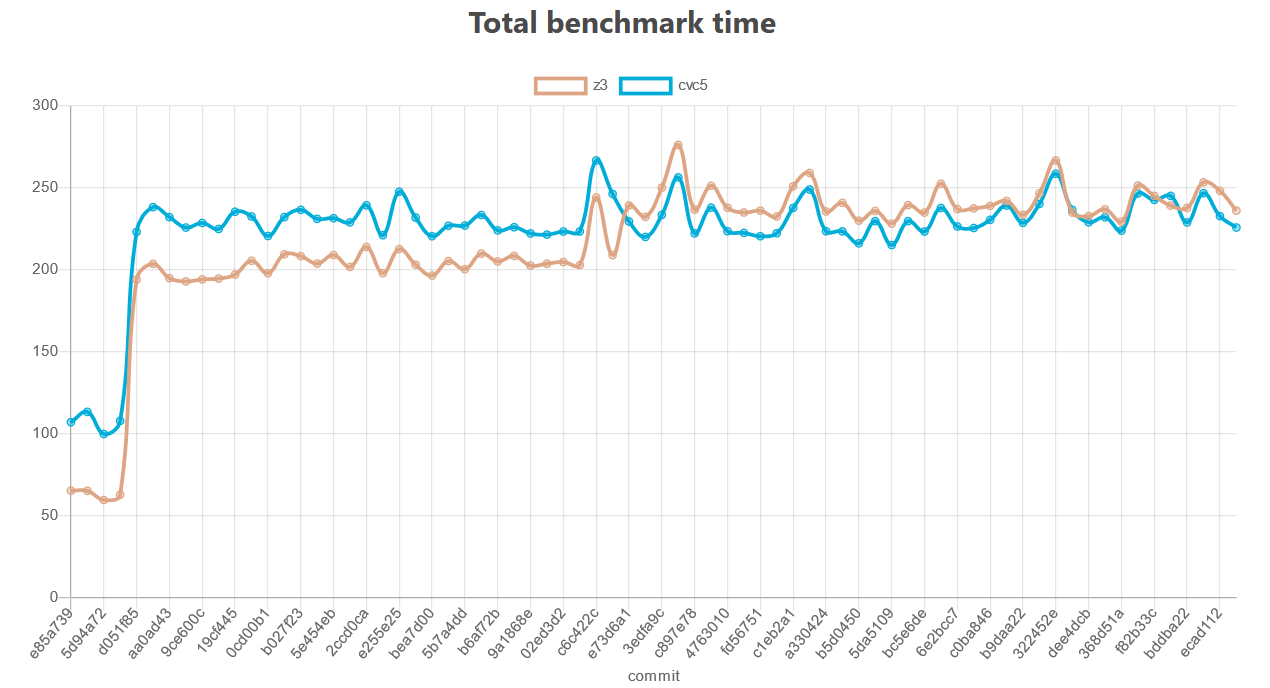
\includegraphics[width=\textwidth]{../misc/vip-performance-hit.png}
    \caption{Sharp increase in execution time when enabling VIP, courtesy of
        \url{https://rems-project.github.io/cerberus/dev/bench/}.}\label{fig:vip-performance-hit}
\end{figure}

Aside from performance, at this stage, it also became clear that not supporting
provenance in bytes was unworkable \textemdash{} 19 out of 44 tests required
additional \cinline{copy_alloc_id} annotation to work as intended. Lack of
support for round-trip was also an issue, this affected 2 tests.

\begin{itemize}
    \item Support memory bytes.
    \item Support \cinline{memcpy}, \cinline{malloc} and \cinline{free}.
    \item Support comparable bytes for \cinline{memcmp}.
    \item Support round-trip casts.
\end{itemize}

\section{Definition of allocation history}

An allocation history is a map from \kl{allocation ID}s (non-empty provenances) to a
record of a base address and a size.

This is reflected in the definition of the \mintinline{ocaml}{Alloc.History}
module, below. Symbols are unique identifiers used to resolved names
immediately after parsing, whereas identifiers are wrappers around strings for
things like names of record fields. I omit the definition of the helper function
\mintinline{ocaml}{make_value} for space. Because I separate the intuitionistic
and linear facts about the allocation history, this is all that is required to
declare it.

\ocamlfile{code/alloc_history.ml}

This is brought into the `empty' typing context, so that it is always in scope
for checking any function, which simply adds the symbol, its type, and some
location information (a built-in variable). Notably, there are no constraints
on it at the beginning.

\ocamlfile{code/empty_context.ml}

\section{Definition of \cninline{Alloc} token}

A definition of a predicate is a record of a location, a symbol for the first
pointer argument, a list of any other input arguments, a type for the output
argument, and an optional list of clauses (the body, potentially guarded by a
series of top-level ifs). The clauses represent the contents of the predicate,
if it can be unfolded (\cninline{Owned} and \cninline{Block} are built-in and
so cannot be unfolded).

\ocamlfile{code/definition_predicate.ml}

Using this, an \cninline{Alloc} token is defined simply as a predicate which
takes only the special pointer argument, no other input arguments, outputs the
record of base address and size, and has no clauses, i.e.\ cannot be unfolded.

\ocamlfile{code/definition_alloc.ml}

This is registered in an environment of definitions and declarations, in the
\ocamlinline{Global} module. Unlike the previous environment, this one does not
change during the course of type checking, but is populated on a per-file
basis. The symbol for \cninline{Alloc} tokens is mapped to the definition
mentioned earlier.

\ocamlfile{code/global_alloc.ml}

The Cerberus front-end supports an extension point, so that the
\cninline{Alloc} token, the \cninline{allocs} logical variables, and other
built-in symbols can be resolved correctly.

\section{Using \cninline{Alloc} in \coreinline{create} and \coreinline{kill}}

These constructs are introduced either by the user, or by a \coreinline{create}
action. Whilst in the formalisation the rules for memory actions are very
clearly synthesising, in the implementation they are more mixed, where terms
are synthesised, but base types are checked, and the contexts are changed along
the way.

The \coreinline{create} action takes as its arguments a pure expression for expressing
the alignment new allocation \ocamlinline{pe}, a C type \ocamlinline{act} and some
source location information \ocamlinline{prefix}. The latter is used only to generate
a helpful name for the logical variable representing the returned pointer.

First the base types are checked to line up, and then the alignment expression.
The continuation for checking the alignment expression names the result as
\ocamlinline{arg}, which is used to create the alignment value
\ocamlinline{align_v}. The return value \ocamlinline{ret} is defined, and a
fresh symbol is created \ocamlinline{ret_s} and added to a (unified) variable
context using \ocamlinline{add_a}. The function \ocamlinline{add_c} add the
constraint that the return value \ocamlinline{ret} is aligned to
\ocamlinline{align_v} to the constraint context. Similarly, \ocamlinline{add_r}
adds the uninitialised ownership resource to the resource context.

\ocamlfile[lastline=18]{code/check_create.ml}

After that, the VIP related code begins. To express bounds constraints on the
new allocation, a constraint that the value keyed by the pointer (actually its
provenance) in the allocation history will equal a record of the return address
and C type size. Note that this constraint is added under a flag
\ocamlinline{use_vip} (the `!' in OCaml is for reading a (mutable) reference,
not for negation). The allocation token is added immediately afterwards. The
typing context logs this action for error reporting, and then passes the
resulting value to an explicit continuation \ocamlinline{k}.

\ocamlfile[firstline=19]{code/check_create.ml}

\section{SMT representation of pointers}

Allocation IDs (non-empty provenances) have their SMT representation
switchable. If VIP is enabled, the representation is just an integer, otherwise
it is the empty tuple.

\ocamlfile[lastline=4]{code/solver_pointer.ml}

Pointers build on this switchable representation, so do not need a switch
themselves. Their SMT representation is a datatype named
\ocamlinline{"pointer"}, which is not polymorphic \ocamlinline{[]}, with two % chktex 18
constructors \ocamlinline{NULL} (which takes no arguments) and
\ocamlinline{AiA} for `\kl{allocation ID} and address' which takes two arguments,
\ocamlinline{"alloc_id"} of type \ocamlinline{CN_Alloc_Id.t ()} and % chktex 18
\ocamlinline{"addr"} of type bit vector (of a width determined by the memory % chktex 18
interface).

\ocamlfile[firstline=20]{code/solver_pointer.ml}

\section{Array and member shifting}

I will only show the code for member shifting; the code for array shifting is
very similar.

Bounds check constraints are as expect \textemdash{} a lookup in the
allocation history followed by constraints that the address of the pointer
(assumed to have an \kl{allocation ID}) must be between the base and base plus
size.

\ocamlfile[lastline=8]{code/check_member_shift.ml}

Having created the constraints, the check for the bound and liveness are gated
by the flag to enable VIP or not. First, it checks the allocation is live.
Next, if the SMT solver can prove the bounds check statically, based on the
available constraints, it will quietly succeed, if not, it will raise an error
saying the allocation for \ocamlinline{term}, is out of bounds
(\ocamlinline{constr} could not be proven), resulting in the \kl{UB} specified
by \ocamlinline{ub}, with \ocamlinline{model} as the counter-example.

\ocamlfile[firstline=10,lastline=24]{code/check_member_shift.ml}

The member shift constructor takes as its arguments a \ocamlinline{pe}
representing the struct address to shift, the struct type \ocamlinline{tag},
and the field \ocamlinline{member}. After the base types are checks, and
\ocamlinline{pe} has been type checked and symbolically evaluated to
\ocamlinline{vt} (value term), first it is checked to have an \kl{allocation ID}
(not be \cinline{NULL}), then, (assuming strict pointer arithmetic), checked to
be in bounds of a live allocation.\sidenote{As explained in the comment in the
code, this check is technically redundant because the elaboration guarantees
that every use of \coreinline{member_shift} is preceded by a call to
\coreinline{PtrValidForDeref}, which checks that the pointer is live and
strictly within bounds (not one past). However, since relying on this is a bit
fragile, I implement the checks anyway.}

\ocamlfile[firstline=26]{code/check_member_shift.ml}

\section{Adding \cinline{copy_alloc_id}}

Checking \cinline{copy_alloc_id} has a similar pattern. It checks the base
types, checks and symbolically evaluates the two arguments. After it does so,
it checks the pointer is not \cinline{NULL}, and then checks the resulting
pointer is in bounds of a live allocation.

\ocamlfile{code/check_copy_alloc_id.ml}

\section{Adapting the PNVI/VIP test suite for CN}

I had to adapt the PNVI/VIP test suite to run with CN in a few ways. First,
because \kl{CN} does not (yet) support \cinline{printf}, I replaced the print
statement with assertions about the expected values at that point in the
program.

Secondly, some of the tests were intended to trigger the non-deterministic
pointer equality. It is not possible to write an assertion that a value
is \emph{not} constrained, and so for that, I used macros
(\cinline{NON_DET_TRUE} and \cinline{NON_DET_FALSE}) as a switch. I show the
example from \cref{fig:nd-ptr-eq-example}, adapted to test CN VIP, below.

\cfile[fontsize=\footnotesize,breaklines]{code/provenance_equality_global_yx.nondet.c}

In addition to checking a variable is \emph{not} constrained, I also needed to
check that some tests fail without \cinline{copy_alloc_id} annotations, and
pass with them. An example of this below, is using exclusive-or to manipulate
and reconstruct and valid pointer address via an integer. Under VIP, the only
way to recover its provenance is to use \cinline{copy_alloc_id}, so the test
must be run both ways to ensure it errors and succeeds appropriately.

\cfile[fontsize=\footnotesize,breaklines]{code/pointer_offset_xor_auto.annot.c}

Finally there are tests which should just pass with no annotations, which I
omit for space.

\section{Non-deterministic pointer equality}

I implement pointer equality and pointer inequality using the same function and
a flags for when the differences arise. In particular, after the base types are
checked, the continuation is re-bound to take the negation of the value at the
end in the negated case.

\ocamlfile[lastline=5]{code/check_ptreq.ml}

After the two operands are checked and symbolically evaluated to
\ocamlinline{arg1} and \ocamlinline{arg2}, I define a helper function to create,
constrain and return a variable.

\ocamlfile[firstline=6,lastline=13]{code/check_ptreq.ml}

I then define the circumstances under which the result is ambiguous: when both
pointers have \kl{allocation ID}s, differing provenances but equal addresses.

\ocamlfile[firstline=14,lastline=27]{code/check_ptreq.ml}

If the solver cannot statically rule out the ambiguous case, a warning is
issued to the user.

\ocamlfile[firstline=28,lastline=41]{code/check_ptreq.ml}

The true case, when both pointers are equal, is easy to define as a constraint.

\ocamlfile[firstline=42,lastline=44]{code/check_ptreq.ml}

The false case, is defined by negation \textemdash{} neither the both-equal
case, nor the ambiguous case.

\ocamlfile[firstline=45,lastline=49]{code/check_ptreq.ml}

Unlike other rules, the result in this case is not a value, a boolean variable
which is constrained to be true in the both-equal case, and to be false in the
neither-equal-nor-ambiguous case. I do not need to state the contrapositive
implications since SMT solvers assume a classical logic. The ambiguous case
leaves the result under-determined by omission, and the result is passed to the
continuation.

\ocamlfile[firstline=50]{code/check_ptreq.ml}

\section{Checking whether a pointer is live}

A check for a live allocation can end in finding a live resource, not finding
one because the resource context has no ownership or allocation tokens, and not
finding one because there was no match (thus resulting in a counter-example).

\ocamlfile[lastline=8]{code/inference_liveness.ml}

Given a resource, an accumulator \ocamlinline{found}, and a candidate pointer
with an \kl{allocation ID} \ocamlinline{res_ptr}, if an answer has already been
found, then skip past this resource, otherwise check if the solver can
statically prove the searched pointer \ocamlinline{ptr} and it have the same
\kl{allocation ID}\@. If that is the case, then signal a resource has been found,
otherwise save the counter-example from the failed proof attempt.

\ocamlfile[firstline=9,lastline=22]{code/inference_liveness.ml}

Given a resource, and an accumulator \ocamlinline{found}, if the resource is
ownership or an allocation token, then check use the pointer from that resource
as a candidate for checking whether it and the search pointer have equal
\kl{allocation ID}s.

\ocamlfile[firstline=23,lastline=36]{code/inference_liveness.ml}

This function is folded over the entire resource context, and missing live
allocations are signalled as errors, with or without the most recent
counter-example.

\ocamlfile[firstline=37]{code/inference_liveness.ml}

\section{Deriving disjointness and bounds constraints on pointers}

One unexpectedly inconvenient aspect of pointers which are partly concrete is
that disjointness facts are expressed over intervals rather than points. This
means that the `distinct' operator provided by some SMT solvers is not
useful.

This means that such facts must be derived from the resource context. For
example, for a single ownership in the context, we may deduce that (a) it has
an \kl{allocation ID} (is not \cinline{NULL}), that the range of addresses it
owns does not wrap-around (the base is less than its upper bound), and that, if
\kl{VIP} is enabled, there exists an allocation which contains it.

\ocamlfile[lastline=15]{code/resource_derived_lc.ml}

Similarly, if \kl{VIP} is enabled and an \cninline{Alloc} token is in the
resource context, we may deduce the intuitionistic constraints associated with
it: the output argument of that resource is the same as the lookup in the
\cninline{allocs} allocation history keyed by the allocation ID of its pointer,
and that the allocation does not wrap-around. Other constraints, including iterated
constraints, do not have any constraints derived from them \textemdash{} this is
likely to need to
change.\sidenote{\url{https://github.com/rems-project/cerberus/issues/541}
    shows that users would like to have disjointness information inferred from
    iterated ownership.}

\ocamlfile[firstline=16,lastline=23]{code/resource_derived_lc.ml}

Constraints may also be derived from pairs of resources in the context, such as
the fact that simultaneous ownership implies the range of owned addresses are
disjoint.\sidenote{This is one of the few places in \kl{CN} that disjunctions
constraints are added to the context.}

\ocamlfile[firstline=25,lastline=35]{code/resource_derived_lc.ml}

Deriving constraints is necessary for soundness but incurs a non-trivial
performance penalty. Hence, there is a flag for disabling it (experimental).
Care must also be taken to not re-derive the same facts, since this also seems
to result in a performance hit to the SMT
solver.\sidenote{\url{https://github.com/rems-project/cerberus/pull/436}}

\ocamlfile[firstline=37]{code/resource_derived_lc.ml}

The facts are derived every time a new resources is added to the context.
They are added to the constraint context because they need to persist,
even if the resource is consumed (for example, consuming ownership
of two pointers does not change the fact that they were and still
are unequal).

\ocamlfile{code/typing_add_r_internal.ml}

\section{Basic support for \cinline{memcpy}}

\section{Insufficiency of not tracking provenance in bytes or integers}

\section{Memory bytes and their use in \coreinline{memcpy}, \coreinline{malloc} and \coreinline{free}}

\section{Comparable bytes in \coreinline{memcmp}}

\section{Integer with/out provenance union type for round-trip casts}

\section{Translating resource lemmas}\label{sec:trans-res-lemmas}

Is there a reason, in the discussion about Cassia's PhD, we thought all of
Cerberus needed to be shoved into Iris instead of just a trace of memory model
(and eventually, concurrency) events?

irisification (cf
\url{https://people.mpi-sws.org/~dreyer/papers/iris-ground-up/paper.pdf}).  Either
just the resource algebra or (as DM suggests) also the abstract language of
memory model interface events: which one let one formalise the primitive
resource-context manipulations that CN does (conceivably extractably).

I think a sufficient halfway point would be the language of traces memory
events i.e.\ memory model as the dynamics. Resource algebra would be CN's view
of resources. Resource lemmas are then just statements saying that one resource
represents exactly the same heap as another resource (skips). Changes to the
resource algebra because of memory events (which we could introduce unsoundness
in CN) would be proved sound in Iris.

As a bonus, we could even formalise and prove sounds the inference procedures
CN uses (and with some engineering to handle SMT, even extract from Rocq).

The inference I'm talking about is resource context manipulations: checking if
we can pack or unpack predicates, if an owned is in the context, shifting
indices in and out of iterated predicates, exploding and imploding structs.
These operations don't require core structure.

Even if full extraction of the inference algo is not feasible (it would
involves standard data structures + SMT FFI), having a defined set of resource
manipulation primitives proved sound and extracting those (just standard data
structure manipulations), or even just proving the primitives sound and using a
similar interface would increase confidence.

If ones reads the above in reverse, it even provides a gradual migration path
which doesn't commit us to any next step and allows us to see how far
extraction can take us.

If the inference algs or the primitives are formalised, then we can iterate on
cleverer  inference schemes with a strong safety net

I think it will become more valuable as soon as we start having fancier things
like higher-order resources, locks, fractional permissions. At that point,
checking the steps/moves that any inference algorithm could take would get
closer to essential.

Even if an arbitrary inference algorithm is not stable, the steps available and
the shape of the resources should be more so, and that is worth at least
creating a clean abstraction for (and then pen-paper soundness, and then
mechanised soundness).

Noted and agreed that anything mechanised takes longer than one wants/expects
and that extraction is a pain. But this gives us a concrete use-case,
reasonable sequence of experiments and a clear idea of the benefits and costs.

